\section{System architecture and Algorithms} \label{sec:Algorithms}

\begin{figure}
%\begin{minipage}{.64\textwidth}
\centering
    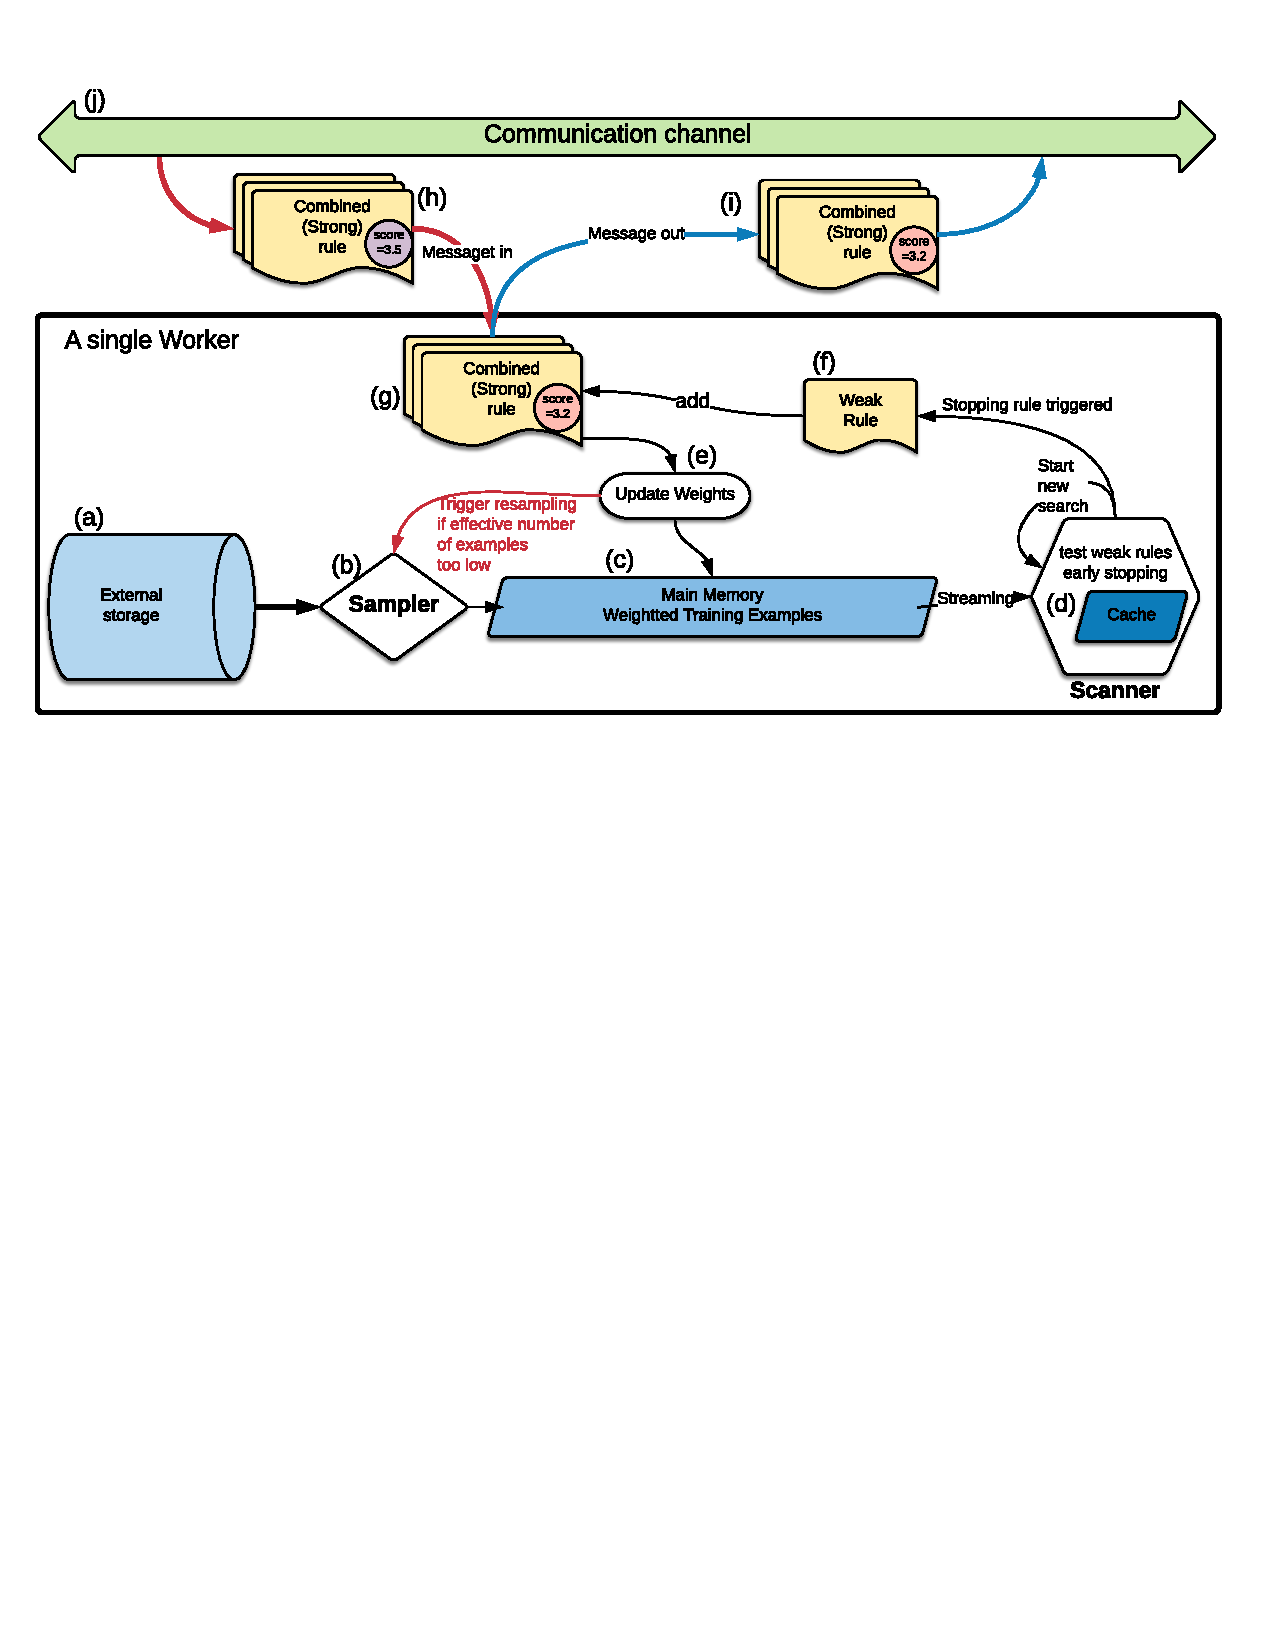
\includegraphics[width=0.7\textwidth]{architecture.pdf}
    \caption{The \Sparrow\ system architecture.}\label{fig:architecture}
    \vspace{0pt}
%\end{minipage}
\end{figure}

The \Sparrow\ distributed system consists of a collection of independent workers
connected through a shared communication channel. There is no
synchronization between the workers and no identified ``head node'' to
coordinate the workers. The result is a highly resilient system in which
there is no single point of failure and the overall slowdown resulting
from machine slowness or failure is proportional to the fraction of
faulty machines.

Each worker is responsible for a finite (small) set of weak
rules. This is a type of feature-based
parallelization~\cite{caragea_framework_2004}. The worker's task is to
identify a weak rule, based on one of the features in the set, that has
a significant edge.

We assume each worker stores {\em all} of the training examples
on it's local disk (element {\bf (a)} in Figure~\ref{fig:architecture})\footnote{In other
  words, the training data it replicated across all of the
  computers. This choice is made to maximize accuracy. If the data is
  too large to fit into the disk of a single worker, then it can be
  randomly partitioned between the computers. The cost is a potential increase
  in the difference between training error and test error}.

Our description of \Sparrow\ is in two parts. First, we describe the
design of a {\em single} \Sparrow\ worker. Following that, we describe
how concurrent workers use the \tmsn\ protocol to update each
other. Figure~\ref{fig:architecture} depicts the architecture of a
single computer and its interaction with the communication
channel. Pseudocode with additional detail is provided in the
supplementary material to this paper.

\subsection{A single \Sparrow\ worker}
\label{sec:single_worker}
As was said above, each worker is responsible for a set of the weak
rules.  The worker's task is to identify a rule that has a significant
edge (Equation~\ref{eqn:gamma_emp}). The worker consists of two
subroutines that can execute in parallel: a {\bf Scanner (d)} and a
{\bf Sampler (b)}. We describe each subroutine in turn.
\paragraph*{The Scanner}(element {\bf (d)} in
Figure~\ref{fig:architecture})
The Scanner's task is to read training examples sequentially and stop
when it has identified one of the rules to be a {\em good} rule. More
specifically, at any time point the Scanner stores the current strong
rule $H_t$, a set of candidate weak rules $\weakRules$ (which
define the candidate strong rules of \tmsn) and a target
edge $\gamma_t$. The scanner scans the training examples stored in
memory sequentially, one at a time. It computes the weight of the
examples using $H_t$ and then updates a running estimate of the edge
of each weak rule $h \in \weakRules$.

The scan stops when the stopping rule determine that
the true edge of a particular weak rule
$\gamma(h_t)$ is, with high probability,
larger than a threshold $\gamma$. The
worker then adds the identified weak rule $h_t$ {\bf (f)} to the current
strong rule $H_t$ to create a new strong rule $H_{t+1}$ {\bf (g)}.

The worker computes a ``performance score'' $z_{t+1}$ which is an
upper bound on the $Z$-score the strong rule by adding the weak rule
to it. The pair $(H_{t+1},z_{t+1})$ is broadcast to the other workers
{\bf (i)}. The worker then resumes it's search using the strong rule
$H_{t+1}$.
\paragraph*{The Sampler} Our assumption is that the entire training dataset does
not fit into main memory and is therefore stored in external storage
{\bf (a)}. As boosting progresses, the weights of the examples become
increasingly skewed, making the dataset in memory effectively smaller.
To counteract that skew, the {\bf Sampler} prepares a {\em new}
training set, in which all of the examples have equal weight, by using
selective sampling. When the effective number of examples associated
with the old training set becomes too small, the scanner stops using
the old training set and starts using the new one.\footnote{The
  sampler and scanner can run in parallel on separate cores. However in
  our current implementation the worker alternates between Scanning and
  sampling.}

The sampler uses selective sampling by which we mean that the
probability that an example $(x,y)$ is added to the sample is
proportional to $w(x,y)$. Each added example is assigned an initial
{\bf weight} of $1$.
\footnote{There are several known algorithms
  for selective sampling. The best known one is rejection sampling
  where a biased coin is flipped for each example. We use a method
  known as ``minimal variance sampling''~\cite{kitagawa_monte_1996}
  because it produces less variation in the sampled set.}
\paragraph*{Incremental Updates:} Our experience shows that the most
time consuming part of our algorithms is the computation of the
predictions of the strong rules $H_t$. A natural way to reduce this
computation is to perform it incrementally. In our case this is
slightly more complex than in XGBoost or LightGBM, because {\bf
  Scanner} scans only a  fraction of the examples at each
iteration. To implement incremental update we store for each example,
whether it is on disk or in memory, the results of the latest
update. Specifically, we store for each training example the tuple
$(x, y, w_s, w_l,H_l)$, Where $x,y$ are the feature vector and the
label, $H_l$ is the strong rule last used to calculate the weight of
the example. $w_l$ is the weight last calculated, and $w_s$ is
example's weight when it was last sampled by the sampler. In this way
{\bf Scanner} and {\bf Sampler} share the burden of computing
the weights, a cost that turns out to be the lion's share of the total
run time for our system.

\subsection{Communication between workers}
Communication between the workers is based on the \tmsn\ protocol.
As explained in Section~\ref{sec:single_worker}, when a worker
identifies a new strong rule, it broadcasts $(H_{t+1},z_{t+1})$ to all
of the other workers. Where $H_{t+1}$ is the new strong rule and
$z_{t+1}$ is an upper bound on the true $Z$-value of $H_{t+1}$. One
can think of $z_{t+1}$ as a ``certificate of quality'' for $H_{t+1}$.

When a worker receives a message of the form $(H,z)$,
it either accepts or rejects it. Suppose that the worker's current
strong rule is $H_t$ whose performance score is $z_t$. 
If  $z_t < z$ then the worker interrupts the Scanner and restarts it
with $(H_t,z_t) \gets (H,z)$.  If $z_t \geq z$ then $(H, z)$ is discarded
and the scanner continues running uninterrupted.

